\clearpage\secrel{Low-level architecture}

\emph{This system primarily targeted for tiny embedded devices},\\
so \textcolor{red}{u\F\ is 16 bit only}. To do it usable toy on large
computers\note{Android is good candidate to play on mobile phone} it is not
required to be big\ --- remember old friendly home computers having not more
than 64K of RAM. In fact, \textcolor{red}{\F\ blew the best platform for
this language}: ZX Spectrum and Commodore 64.

\smallskip\noindent
\begin{tabular}{l l l}
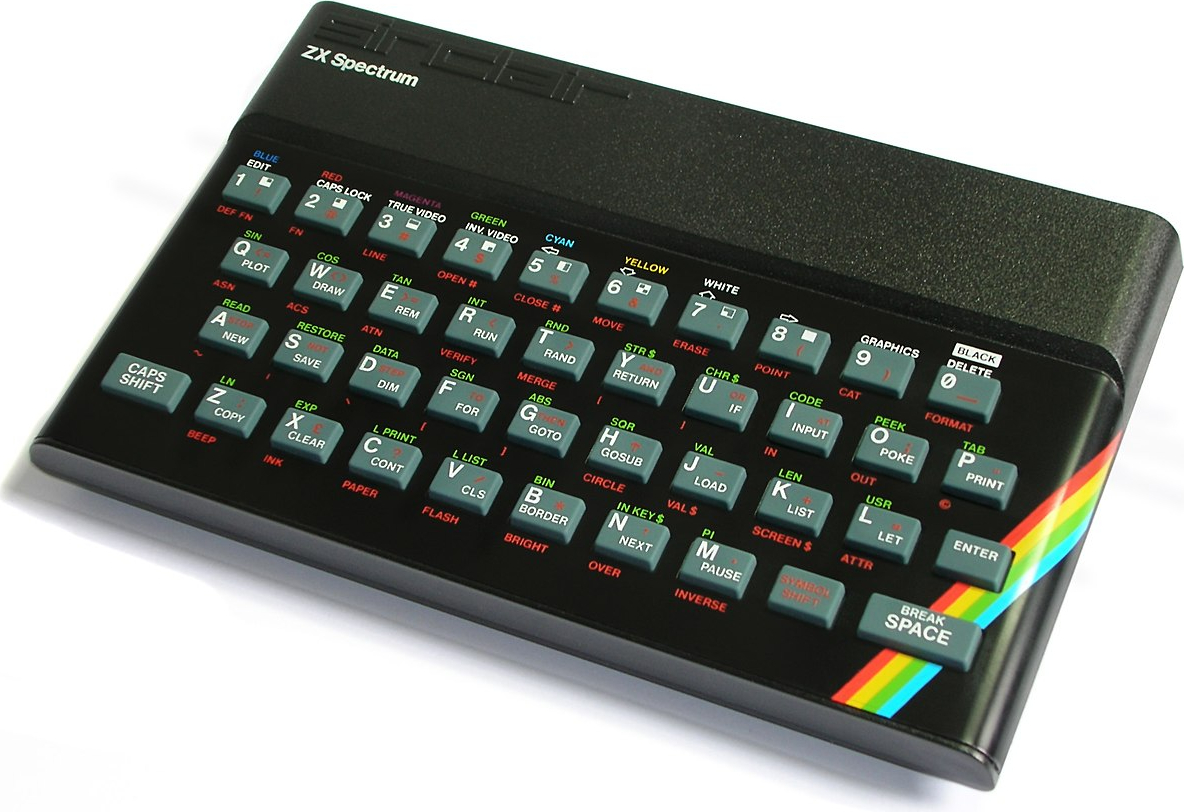
\includegraphics[height=0.35\textheight]{img/ZX48.jpg} &
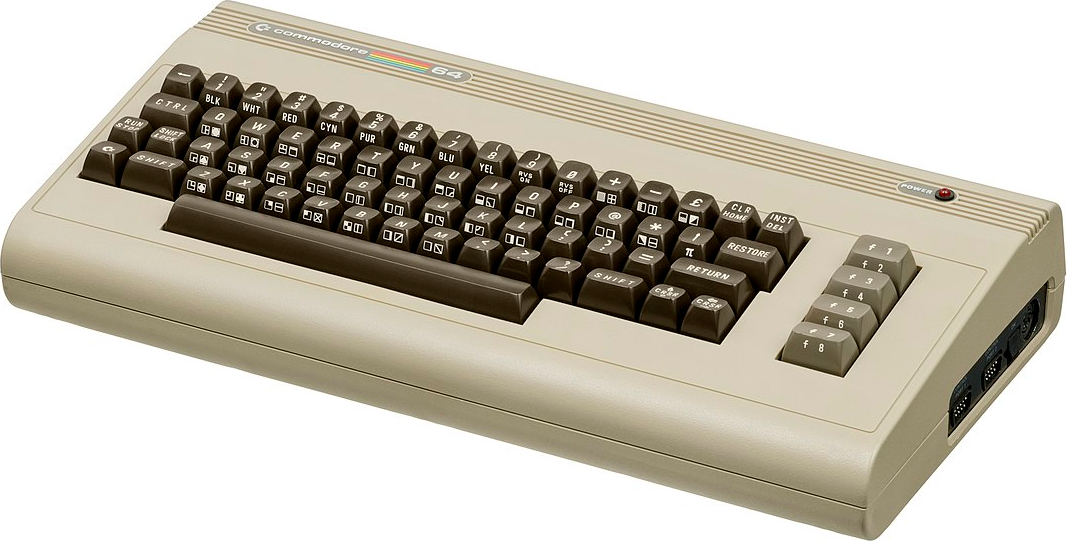
\includegraphics[height=0.35\textheight]{img/C64.jpg} &
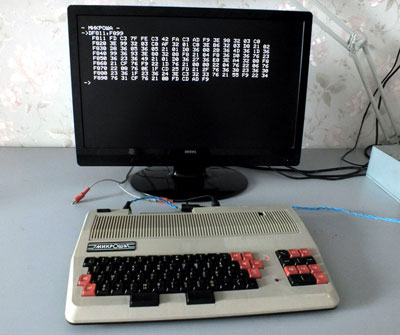
\includegraphics[height=0.35\textheight]{img/microsha.jpg} \\
\end{tabular}
\clearpage

\noindent
This tiny computers was totally (!) conformant to \F:
\begin{itemize}[nosep]
  \item few RAM starting from 16K, and not more then 64K\\
  (some latest models had 128K)
  \item tiny 8bit cheap processor: i8080, Z80, 6502
  \item user must be able to program it using ROM firmware\\using easy
  high-level programming language
  \item real programs must be written in assembly because of lack of RAM
  and CPU power
  \item direct access to hardware: strange framebuffer and i/o ports
\end{itemize}
BASIC was selected for learning, but \emph{all these computers allow to replace
ROM} chip or use external pluggable ROMs. And FORTH fails the same way as
SmallTalk: \textcolor{red}{price kills the language feature}.

\clearpage

\noindent
Notably, this \term{deskboard computer formfactor} still \emph{can be accepted
by consumer market}. In early days of hobby home computing, the most annoying
problem was keyboard quality: they were ugly. Modern technologies allow making a
good quality keyboard with embedded SoC power enough to process multimedia
without any lags and do good gaming graphics in hardware level. Large casing
lets to use modern multicore mobile SoCs from MTK and AllWinner with OpenGL
and large RAM, without any problems of overheating. Backside able to carry all
required interfaces: Ethernet, HDMI+VGA, and huge USB hub.
Other variant is \emph{extra cheap computers}: STM32F7 MCU family
have enough interfaces and computing power to be good in this old style cheap
consoles.

\clearpage

\begin{lstlisting}[language=C]
/* sizes of statically allocated structures */
#define Dsz 0x10
#define Rsz 0x100
#define Msz 0x1000

void VM() {}	/* virtual machine startup */

#ifdef EMULATOR
/* this code will be compiled only for emulator */
int main() { VM(); return 0; }
#endif
\end{lstlisting}
\begin{lstlisting}[language=C]
#include <stdint.h>						/* std.includes */
#ifdef EMULATOR ...	/* for emulator mode only */

/* set 16/32 bit mode
	CELL is machine word for FORTH systems */
#define  CELL  int16_t /* light microcontrollers */
#define UCELL uint16_t

/* data stack */
 CELL D[Dsz]; uint16_t Dp=0; /*[D]ata [p]ointer*/
/* return stack */
UCELL R[Rsz]; uint16_t Rp=0; /*[R]eturn [p]ointer*/
\end{lstlisting}

